\chapter{Application Layer: Parallel Programming API} \label{sec:api}

\section{Background}\label{sec:api:background}

Before discussing how the selected Application Programming interface (API) works, it is necessary that the reader have some familiarity with parallel programming, so this section will first give an introduction to parallel programming before discussing the Message Passing Interface (MPI). Although this chapter focuses on parallel computing, these concepts are equally applicable to distributed computing.

\subsection{Parallel Programming}\label{sec:api:background:parallel_computing}

The first step in designing any parallel algorithm is to identify what parallelisms are inherent in the algorithm at hand. Parallelisms can be divided into two categories: data parallelism and task parallelism. Task parallelism is where different parts of the algorithm can be executed concurrently. Operating systems exhibit task parallelism by executing different programs at the same time. Task parallelism at the algorithm level generally does not scale well because the number of tasks are fixed. Data parallelism is where the same algorithm can be applied to multiple data items concurrently. Media encoders often exploit data parallelism by encoding different parts of the source media concurrently. Data parallelism scales well with data size. As the size of data grows, the parallelisms scale accordingly. Almost all parallel programming exploits data parallelism, and will be the focus of the rest of this chapter. \cite{ref:2009-snyder-principles_of_parallel_programming}

There are three basic methodologies for formulating a parallel computation. In fixed parallelism, a programmer targets a specific machine or cluster with  processors and employs a -way solution. This method is very easy to program, but does not perform any faster on machines with  processors. This method is rarely employed in practice due to its lack of scalability. In unlimited parallelism, a programmer exploits all parallelisms in the algorithm. Traditionally this leads to two related problems: managing more than one thread per processor uses more overhead than a single thread per processor, and communication overhead becomes the dominating time factor. There has been recent work in this area to make this approach tenable, however. Apple, Inc. recently unveiled a technology called Grand Central Dispatch (GCD) that introduces the idea of a lightweight task, called a block, and operates similar to a closure\footnote{In programming language theory, a closure is a first-class function that can use free-variables that are ``private''}. Blocks are queued by the GCD runtime to run on specific processors in an under-the-hood thread. Apple encourages programmers to use unlimited parallelism in their algorithms because the overhead for a block is almost non-existent. \cite{ref:2009-apple-grand_central_dispatch} In scalable parallelism, a programmer identifies all of the ``substantial'' work units to be done (i.e. things that are ``obvious'') and implements mechanisms for distributing these work units to the available processing units. This allows the algorithm to scale up to the number of work units while minimizing overhead. This method is the most predominant, but is also the most difficult to implement correctly. \cite{ref:2009-snyder-principles_of_parallel_programming}

There are four basic sources of performance loss associated with parallel computing. The first is overhead associated with parallelizing the algorithm. Overhead includes communication overhead, synchronization overhead, extra computations associated with making the algorithm parallel, and extra memory required to make the algorithm parallel. The second source of performance loss is computation that cannot be parallelized. Certain types of algorithms are just inherently sequential, such as waiting on I/O. The third source of performance loss is contention for resources. When multiple processors need to access a shared resource, overhead is incurred in arbitrating the requests. The fourth source of performance loss is idle processors. When an algorithm does not distribute work equally, called a load imbalance, processors end up sitting idle while others are working, which reduces efficiency. \cite{ref:2009-snyder-principles_of_parallel_programming}

Non-parallelizable code and resource contention manifest themselves due to ``dependences.'' A dependency in parallel computing is a relationship between tasks that requires those tasks to execute in order. Almost all dependencies are data dependencies, which is an ordering of memory operations. There are three basic types of data dependencies: flow dependence, anti dependence, and output dependence. A flow dependence is a read after write ordering, which requires that one task reads the value that another task writes to memory. If the first task reads out of order, then it will get the wrong value. An anti dependence is basically the opposite of a flow dependence, in which case a task needs to read a value before another task overwrites it. An output dependence requires that one task writes to memory before another task writes to that memory. There is a special class of problems that have no dependencies, often accompanied by a large data set. These problems are called ``embarrassingly parallel.'' \cite{ref:2009-snyder-principles_of_parallel_programming}

Related to dependencies is the notion of ``granularity.'' Granularity, usually defined as ``coarse'' and ``fine,'' specifies the relative frequency of communication between tasks due to dependencies. A coarse grained algorithm contains little communication between tasks, while a fine grained algorithm contains much communication between tasks. Fine grained algorithms are best suited to shared memory systems, where synchronization overhead is pretty low. On the flip side, coarse grained algorithms are best suited to distributed memory systems, where synchronization overhead is much larger. It should be noted that some algorithms can only be parallelized in a fine-grained manner. \cite{ref:2009-snyder-principles_of_parallel_programming}

Speedup is a measurement of how much performance is increased by utilizing parallel computing. Speedup is defined as $S=T\_S/T\_P$, where $T\_S$ is the execution time of the sequential algorithm, and $T\_P$ is the execution time of the parallel algorithm. Speedup is typically measured across a varied number of processor and plotted on a graph. The theoretical speed is typically plotted for reference and is defined as $T\_S/n$ given $n$ processors. There is a curious case where an algorithm will experience ``super-linear'' speedup, that is the speedup is greater than $T\_S/n$. This occurs when the parallel algorithm does less aggregate work than the sequential variant. One common scenario is when the parallel algorithm is able to fit all data in each processors cache but the sequential algorithm cannot, leading to more memory hits. Another common scenario is with a parallel search that terminates as soon as the desired element is found. Efficiency is a measure of how effective the speedup is, and is defined as $S/n$. An efficiency of 1 indicates a perfect speedup. An efficiency above 1 indicates super-linear speedup, and an efficiency below 1 indicates that there is performance loss. \cite{ref:2009-snyder-principles_of_parallel_programming}

When programming a parallel algorithm, it is important that the program is correct, achieves good performance, is scalable to a large number of processors, and is portable across a wide variety of platforms. As this section has shown, there are many competing factors that make it difficult to achieve these goals.

\subsection{Message Passing Interface Overview}\label{sec:api:background:mpi_overview}

The Message Passing Interface (MPI) API is designed primarily for distributed memory systems. MPI provides a set of functions for sending and receiving messages and synchronizing processes, with Fortran, C, and C++ bindings. Programmers almost always use MPI for distributed memory parallel programming when using an existing API. 

MPI uses a mechanism called a ``communicator'' to define scope. All process are part of a default communicator called ``MPI\_COMM\_WORLD,'' but other communicators can be defined as well. Communicators are used by the other functions to define the scope of the operation (think multicast). Communicators can be used to perform task level parallelism, among other things.

MPI provides a variety of sending and receiving options, but the most common are a blocking send/receive and a non-blocking send/receive. The send functions blocks until the message is successfully received at the other end, while a non-blocking send returns immediately to allow other processing to take place. Each send call must have a corresponding receive call on the other end. Receive calls can also be blocking or non-blocking. MPI also includes a broadcast mechanism. When used with a communicator, broadcast behaves like multicast.

MPI provides a barrier function for synchronizing processes. When a process encounters a barrier, it blocks until all other processes have also encountered the barrier. Barriers are useful for working out dependency issues, especially flow dependencies.

MPI provides a number of higher level functions for performing common functions. There are two functions called scatter and gather that tend to work together. Scatter takes a vector, divides it up, and sends each piece out to a different node such that the vector is now scattered around the system. Gather is essentially the opposite of scatter and receives data from all of the nodes in the system and reassembles it into a single vector. There is also a function called reduce that is basically a gather function coupled with some post processing. Available reduction operations include summation, max/min, bitwise and logical Boolean operations, and user-defined operations.

The full MPI specification contains hundreds of functions, although in practice most people only use around a dozen of these functions. MPI was first created in 1994 and is at version 2.2 as of this writing.

\section{Objectives}\label{sec:api:objectives}

As mentioned in Chapter \ref{sec:introduction}, the application layer API must meet the following criteria: 
\begin{itemize}
	\item Implements a subset of the MPI 1.1 specification
	\item All methods that are implemented must be compatible with the existing specification
	\item Must not require the developer to configure anything outside of normal MPI configuration.
\end{itemize}
The basic idea behind these requirements is to ensure that simple MPI programs can be ported to the system with little to no modification.

\section{Methodology}\label{sec:api:methodology}

A total of 11 MPI functions are included in the toolkit as of this writing. These functions provide basic send/receive support, synchronization, and system support. The functions and their descriptions are shown in Table \ref{tab:api:mpi_functions}. The C bindings are shown because the API for the toolkit is written in C. Note that all functions return a status code.

\pagebreak[4]
\begin{longtable}{|p{5.5in}|}

\caption*{MPI functions in the toolkit \cite{ref:2010-llnl-mpi_reference}}\label{tab:api:mpi_functions}
\endfirsthead
\endhead
\endfoot
\endlastfoot

\hline

\vspace{-0.8cm}

\LARGE{\bfseries{MPI\_Init}} \\

\vspace{-0.3cm}

\emph{\bfseries{Definition:}} \\
\lstinline$int MPI_Init(int *argc,char ***argv);$ \\
\vspace{-0.3cm}

\emph{\bfseries{Description:}} \\
This subroutine initializes MPI. All MPI programs must call MPI\_INIT before any other MPI. More than one call to MPI\_INIT by any task results in unspecified behavior. MPI\_INIT blocks until all nodes have initialized. \\
\vspace{-0.3cm}

\emph{\bfseries{Arguments:}} \\
\lstinline$argc$ \\
\hspace{0.5cm}is the number of command-line arguments \\
\lstinline$argv$ \\
\hspace{0.5cm}is the command-line arguments \\
\vspace{-0.3cm}

\emph{\bfseries{Note:}} \\
The arguments are here for compatibility only. They do nothing in the toolkit. \\

\hline

\vspace{-0.8cm}

\LARGE{\bfseries{MPI\_Finalize}} \\

\vspace{-0.3cm}

\emph{\bfseries{Definition:}} \\
\lstinline$int MPI_Finalize(void);$ \\
\vspace{-0.3cm}

\emph{\bfseries{Description: }} \\
This function actually does nothing in the toolkit, but is here for compatibility.\\

\hline

\vspace{-0.8cm}

\LARGE{\bfseries{MPI\_Comm\_size}} \\

\vspace{-0.3cm}

\emph{\bfseries{Definition: }} \\
\lstinline$int MPI_Comm_size(MPI_Comm comm,int *size);$ \\
\vspace{-0.3cm}

\emph{\bfseries{Description: }} \\
This subroutine returns the size of the group associated with a communicator. The size is equal to the number of nodes in the routing tree minus 1 (the root does not participate). \\
\vspace{-0.3cm}

\emph{\bfseries{Arguments: }} \\
\lstinline$comm$ \\
   \hspace{0.5cm}  is the communicator (handle) \\
\lstinline$size$ \\
\hspace{0.5cm}     is an integer specifying the number of tasks in the group of comm \\
\vspace{-0.3cm}

\emph{\bfseries{Note: }} \\
Only communicator MPI\_COMM\_WORLD is supported in the toolkit\\

\hline

\vspace{-0.8cm}

\LARGE{\bfseries{MPI\_Comm\_rank}} \\

\vspace{-0.3cm}

\emph{\bfseries{Definition: }} \\
\lstinline$int MPI_Comm_rank(MPI_Comm comm,int *rank);$ \\
\vspace{-0.3cm}

\emph{\bfseries{Description: }} \\
This subroutine returns the rank of the local task in the group associated with a communicator. You can use this subroutine with MPI\_COMM\_SIZE to determine the amount of concurrency available for a specific job. MPI\_COMM\_RANK indicates the rank of the task that calls it in the range from 0...size - 1, where size is the return value of MPI\_COMM\_SIZE. The rank is equal to the node address minus 2. \\
\vspace{-0.3cm}

\emph{\bfseries{Arguments: }} \\
\lstinline$comm$\\
\hspace{0.5cm}     is the communicator (handle) (IN)\\
\lstinline$rank$\\
\hspace{0.5cm}     is an integer specifying the rank of the calling task in group of comm \\
\vspace{-0.3cm}

\emph{\bfseries{Note: }} \\
Only communicator MPI\_COMM\_WORLD is supported in the toolkit\\

\hline

\vspace{-0.8cm}

\LARGE{\bfseries{MPI\_Send}} \\

\vspace{-0.3cm}

\emph{\bfseries{Definition: }} \\
int MPI\_Send(void* buf,int count,MPI\_Datatype datatype,int dest,int tag,MPI\_Comm comm); \\
\vspace{-0.3cm}

\emph{\bfseries{Description: }} \\
This subroutine is a blocking standard mode send operation. MPI\_SEND causes count elements of type datatype to be sent from buf to the task specified by dest. \\
\vspace{-0.3cm}

\emph{\bfseries{Arguments: }} \\
\lstinline$buf$\\
\hspace{0.5cm}     is the initial address of the send buffer (choice)\\
\lstinline$count$\\
\hspace{0.5cm}     is the number of elements in the send buffer (non-negative integer)\\
\lstinline$datatype$\\
\hspace{0.5cm}     is the datatype of each send buffer element (handle)\\
\lstinline$dest$\\
\hspace{0.5cm}     is the rank of the destination task in comm(integer)\\
\lstinline$tag$\\
\hspace{0.5cm}     is the message tag (positive integer)\\
\lstinline$comm$\\
\hspace{0.5cm}     is the communicator (handle) \\
\vspace{-0.3cm}

\emph{\bfseries{Note: }} \\
Only communicator MPI\_COMM\_WORLD is supported in the toolkit\\

\hline

\vspace{-0.8cm}

\LARGE{\bfseries{MPI\_Recv}}\\

\vspace{-0.3cm}

\emph{\bfseries{Definition: }} \\
int MPI\_Recv(void* buf,int count,MPI\_Datatype datatype,int source,int tag,MPI\_Comm comm,MPI\_Status *status); \\
\vspace{-0.3cm}

\emph{\bfseries{Description: }} \\
MPI\_RECV is a blocking receive operation. The receive buffer is storage containing room for count consecutive elements of the type specified by datatype, starting at address buf. The message received must be less than or equal to the length of the receive buffer. If all incoming messages do not fit without truncation, an overflow error occurs. If a message arrives that is shorter than the receive buffer, then only those locations corresponding to the actual message are changed. \\
\vspace{-0.3cm}

\emph{\bfseries{Arguments: }} \\
\lstinline$buf$\\
\hspace{0.5cm}     is the initial address of the receive buffer (choice)\\
\lstinline$count$\\
\hspace{0.5cm}     is the number of elements to be received (integer)\\
\lstinline$datatype$\\
\hspace{0.5cm}     is the datatype of each receive buffer element (handle)\\
\lstinline$source$\\
\hspace{0.5cm}     is the rank of the source task in comm or MPI\_ANY\_SOURCE (integer)\\
\lstinline$tag$\\
\hspace{0.5cm}     is the message tag or MPI\_ANY\_TAG (positive integer)\\
\lstinline$comm$\\
\hspace{0.5cm}     is the communicator (handle)\\
\lstinline$status$\\
\hspace{0.5cm}     is the status object (Status) \\
\vspace{-0.3cm}

\emph{\bfseries{Note: }} \\
Only communicator MPI\_COMM\_WORLD is supported in the toolkit\\

\hline

\vspace{-0.8cm}

\LARGE{\bfseries{MPI\_Irecv}} \\

\vspace{-0.3cm}

\emph{\bfseries{Definition: }} \\
int MPI\_Irecv(void* buf,int count,MPI\_Datatype datatype,int source,int tag,MPI\_Comm comm,MPI\_Request *request); \\
\vspace{-0.3cm}

\emph{\bfseries{Description: }} \\
This subroutine starts a non-blocking receive and returns a handle to a request object. The request is later used to query the status of the communication or wait for it to complete. A non-blocking receive call means the system may start writing data into the receive buffer. Once the non-blocking receive operation is called, do not access any part of the receive buffer until the receive is complete. \\
\vspace{-0.3cm}

\emph{\bfseries{Arguments: }} \\
\lstinline$buf$\\
\hspace{0.5cm}     is the initial address of the receive buffer (choice)\\
\lstinline$count$\\
\hspace{0.5cm}     is the number of elements in the receive buffer (integer)\\
\lstinline$datatype$\\
\hspace{0.5cm}     is the datatype of each receive buffer element (handle)\\
\lstinline$source$\\
\hspace{0.5cm}     is the rank of source or MPI\_ANY\_SOURCE (integer)\\
\lstinline$tag$\\
\hspace{0.5cm}     is the message tag or MPI\_ANY\_TAG (positive integer)\\
\lstinline$comm$\\
\hspace{0.5cm}     is the communicator (handle)\\
\lstinline$request $\\
\hspace{0.5cm}     is the communication request (handle) \\
\vspace{-0.3cm}

\emph{\bfseries{Note: }} \\
Only communicator MPI\_COMM\_WORLD is supported in the toolkit\\

\hline

\vspace{-0.8cm}

\LARGE{\bfseries{MPI\_Test}} \\

\vspace{-0.3cm}

\emph{\bfseries{Definition: }} \\
int MPI\_Test(MPI\_Request *request,int *flag,MPI\_Status *status); \\
\vspace{-0.3cm}

\emph{\bfseries{Description: }} \\
MPI\_TEST returns flag = true if the operation identified by request is complete. The status object is set to contain information on the completed operation. Otherwise, flag = false and the status object is undefined. The status object can be queried for information about the operation. \\
\vspace{-0.3cm}

\emph{\bfseries{Arguments: }} \\
\lstinline$request$\\
\hspace{0.5cm}     is the operation request (handle)\\
\lstinline$flag$\\
\hspace{0.5cm}     is true if the operation completed (logical)\\
\lstinline$status$\\
\hspace{0.5cm}    is the status object (Status)\\

\hline

\vspace{-0.8cm}

\LARGE{\bfseries{MPI\_Get\_count}} \\

\vspace{-0.3cm}

\emph{\bfseries{Definition: }} \\
int MPI\_Get\_count(MPI\_Status *status,MPI\_Datatype datatype,int *count); \\
\vspace{-0.3cm}

\emph{\bfseries{Description: }} \\
This subroutine returns the number of elements in a message. The datatype argument and the argument provided by the call that set the status variable should match. When one of the MPI wait or test calls returns status for a non-blocking operation request and the corresponding blocking operation does not provide a status argument, the status from this wait or test call does not contain meaningful source, tag, or message size information. \\
\vspace{-0.3cm}

\emph{\bfseries{Arguments: }} \\
\lstinline$status$\\
\hspace{0.5cm}     is a status object (Status)\\
\lstinline$datatype$\\
\hspace{0.5cm}     is the datatype of each message element (handle)\\
\lstinline$count$\\
\hspace{0.5cm}     is the number of elements (integer)\\

\hline

\vspace{-0.8cm}

\LARGE{\bfseries{MPI\_Barrier}} \\

\vspace{-0.3cm}

\emph{\bfseries{Definition: }} \\
int MPI\_Barrier(MPI\_Comm comm); \\
\vspace{-0.3cm}

\emph{\bfseries{Description: }} \\
This subroutine blocks until all tasks have called it. Tasks cannot exit the operation until all group members have entered. \\
\vspace{-0.3cm}

\emph{\bfseries{Arguments: }} \\
\lstinline$comm$\\
\hspace{0.5cm}     is a communicator (handle)\\
\hline
\end{longtable}

\section{Implementation}\label{sec:api:implementation}

Support for MPI has been built directly into the protocol implementation. When data is received via the receive data command, it assumes that the payload is destined for the MPI runtime and sends it on its way. A mail system has been created to provide communication between the protocol and the MPI runtime. The mail system has a queued inbox with the capability to read the next message, or the next message with a specific subject. 

The \lstinline$MPI_Send$ function is currently implemented to handle data transfers consisting of 16-bit integers of arbitrary length. The network layer limits data transfers to 256 bytes, which implies that data transfers longer than that will need to be broken up into multiple transfers. In addition, guaranteed delivery needs to be implemented because the network layer does not guarantee delivery. The process for handling these requirements is shown in Figure \ref{fig:api:send_process_diagram}. The send function first partitions the data into 255 byte chunks. Then, it creates a ``transfer initialization'' packet that contains the reserved packet ID's of the data transfers for each partition. Pre-allocating the packet ID's allows each end of the transfer to monitor the progress and re-request a transfer if there is a packet error or timeout. Every time a packet is received correctly, a ``transfer success'' message is sent to the MPI runtime, and every time there is a transfer error or timeout, a ``transfer failure'' message is sent. This makes it easy for the runtime to determine if a packet has failed or succeeded. Once the transfer success message has been received for the transfer initialization packet, the data partitions can be sent. Each data partition is sent in parallel to help reduce latency in establishing the data transfer. The system then waits for all transfer success messages to be received, re-transferring partitions as the need arises.

\begin{figure}[ptb]
	\begin{centering}
		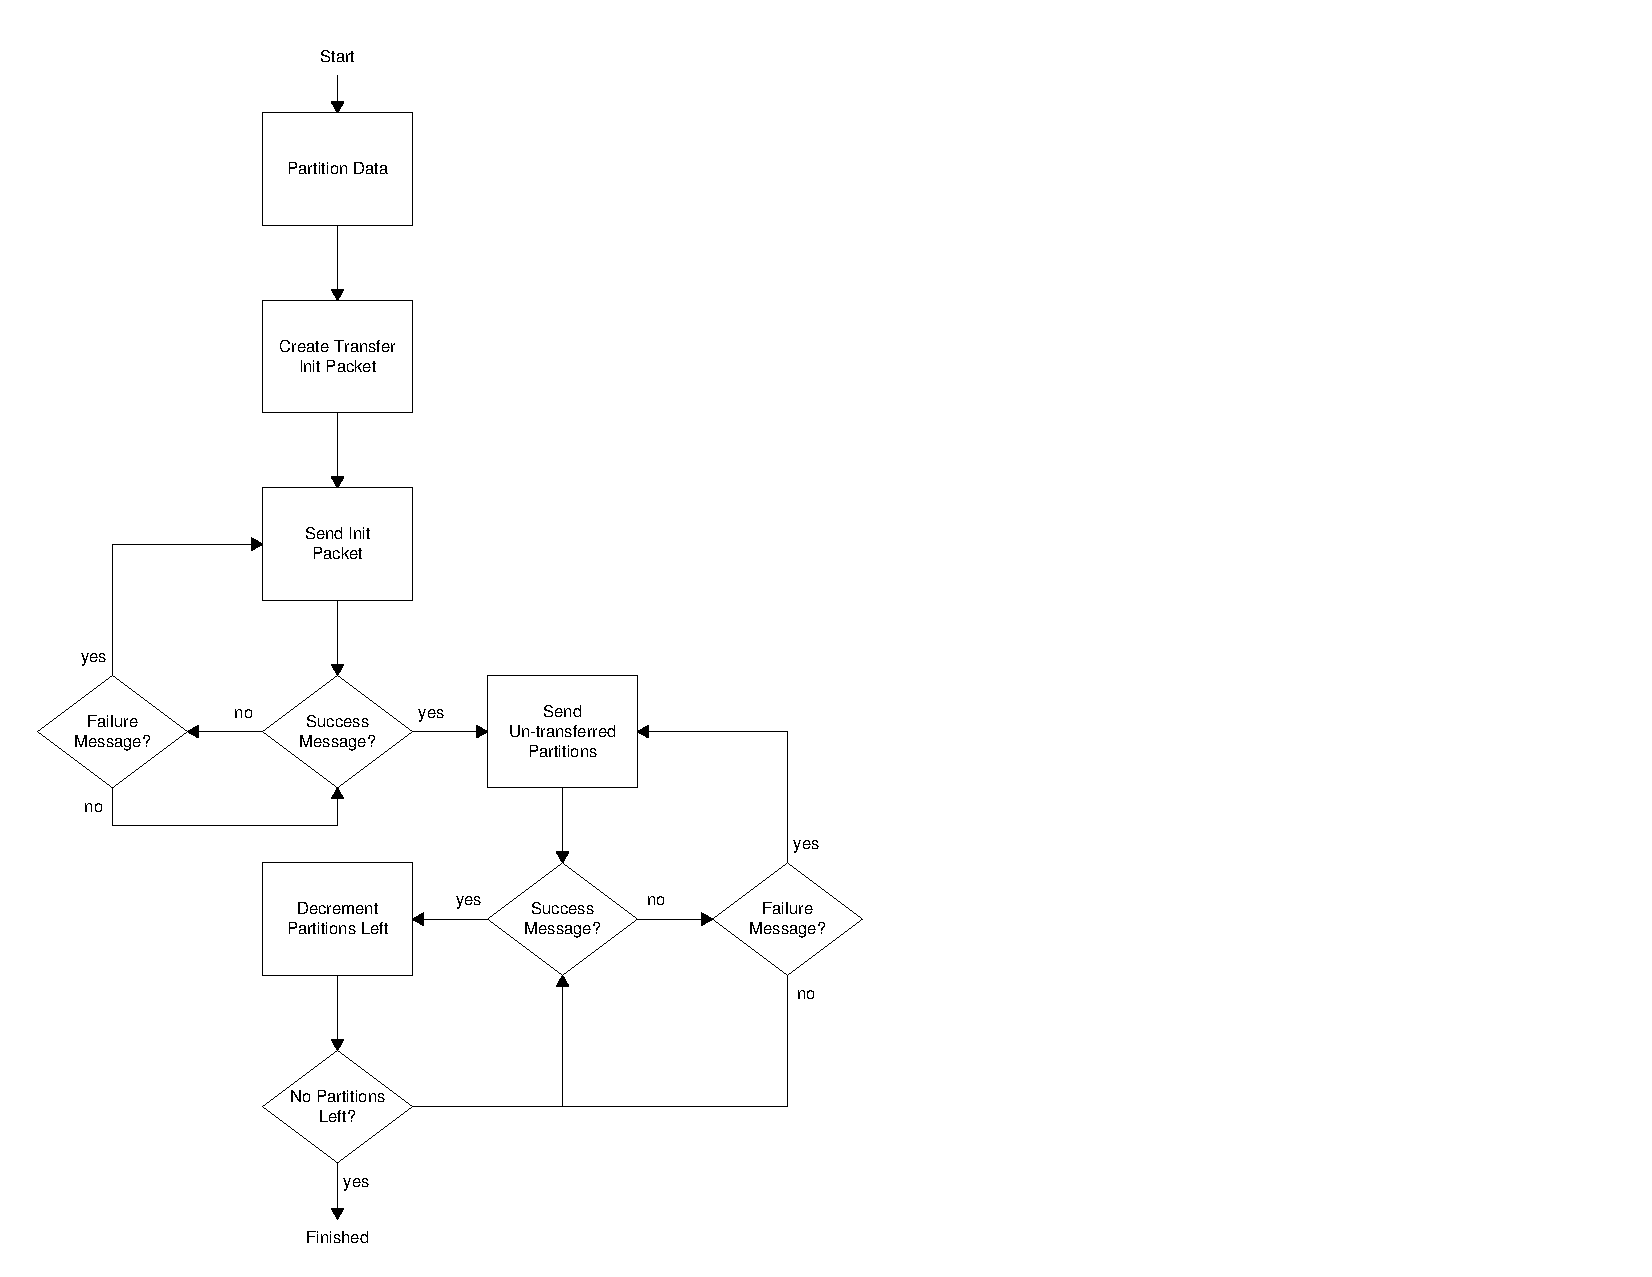
\includegraphics{API/Figures/api-send_process_diagram.pdf}
		\caption{Send Process Diagram}
		\label{fig:api:send_process_diagram}
	\end{centering}
\end{figure}

The \lstinline$MPI_Recv$ function is implemented in two parts: the protocol side and the runtime side. Much of the receive code actually needs to be implemented with the network layer code because receives need to be handled regardless of whether or not the MPI application has called \lstinline$MPI_Recv$. On the protocol side, the code looks for transfer initialization packets. When one is received, the partition info is stored and a data buffer is created to hold the partitions. Note that the partitions are immediately copied to the proper location in the data buffer on receipt. After that, data partitions are saved to the buffer as they are received. Once all of the partitions have been received, a transfer received message is sent to the MPI runtime. On the runtime side, the code simply polls the mailbox continuously until the transfer received message is received. This implements the blocking nature of the function.

\begin{figure}[ptb]
	\begin{centering}
		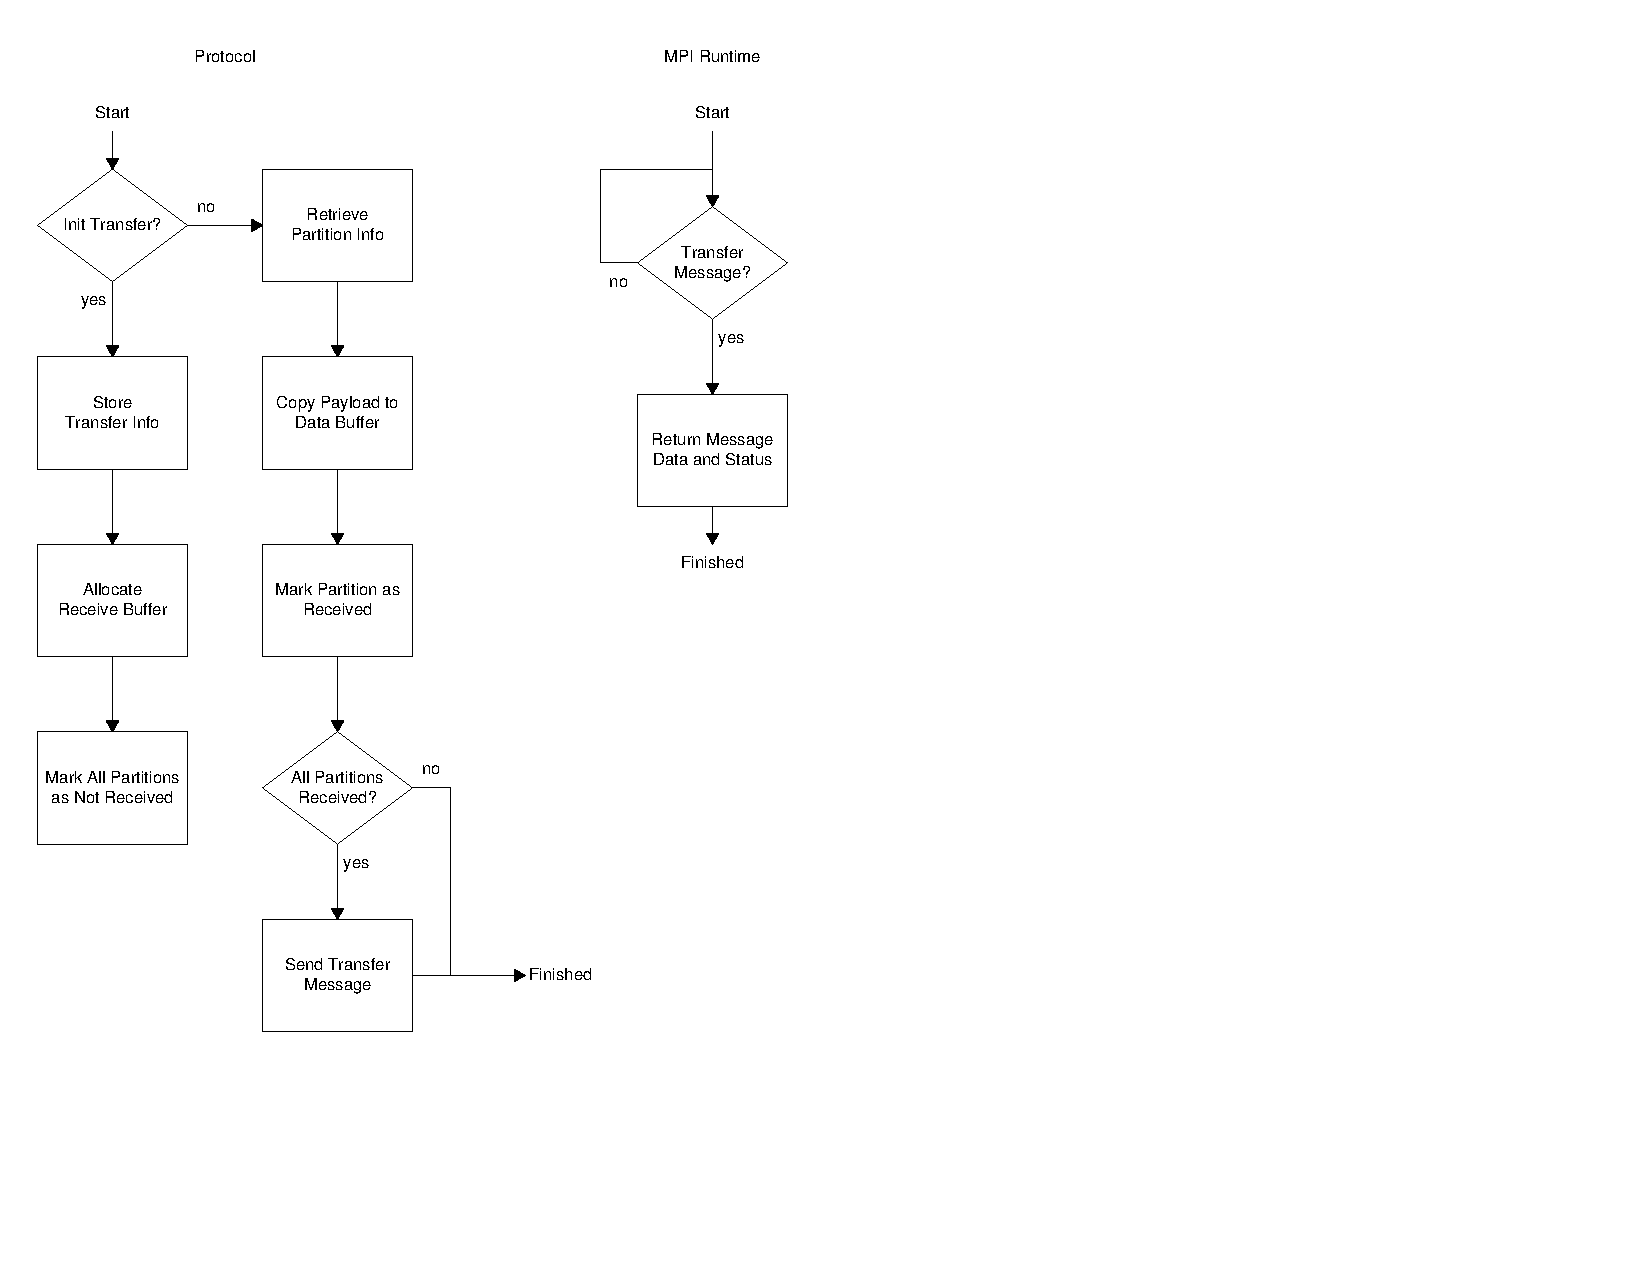
\includegraphics{API/Figures/api-receive_process_diagram.pdf}
		\caption{Receive Process Diagram}
		\label{fig:api:receive_process_diagram}
	\end{centering}
\end{figure}

The \lstinline$MPI_Irecv$ function is almost identical to the \lstinline$MPI_Recv$ function, except that the MPI runtime side code doesn't wait for the mail message. It also sets the status value. Status is a ``black-box'' variable because it is never accessed directly. The MPI specification leaves it up to the MPI implementations to determine its structure. The toolkit uses the status to store the message that was sent from the network layer side code in the event of a successful transfer. A ``no message'' message is used if the transfer hasn't completed yet. The application programmer uses this status in combination with the \lstinline$MPI_Test$ function to see if the transfer has completed and the \lstinline$MPI_Get_count$ to see how big the data transfer was.

\begin{figure}[ptb]
	\begin{centering}
		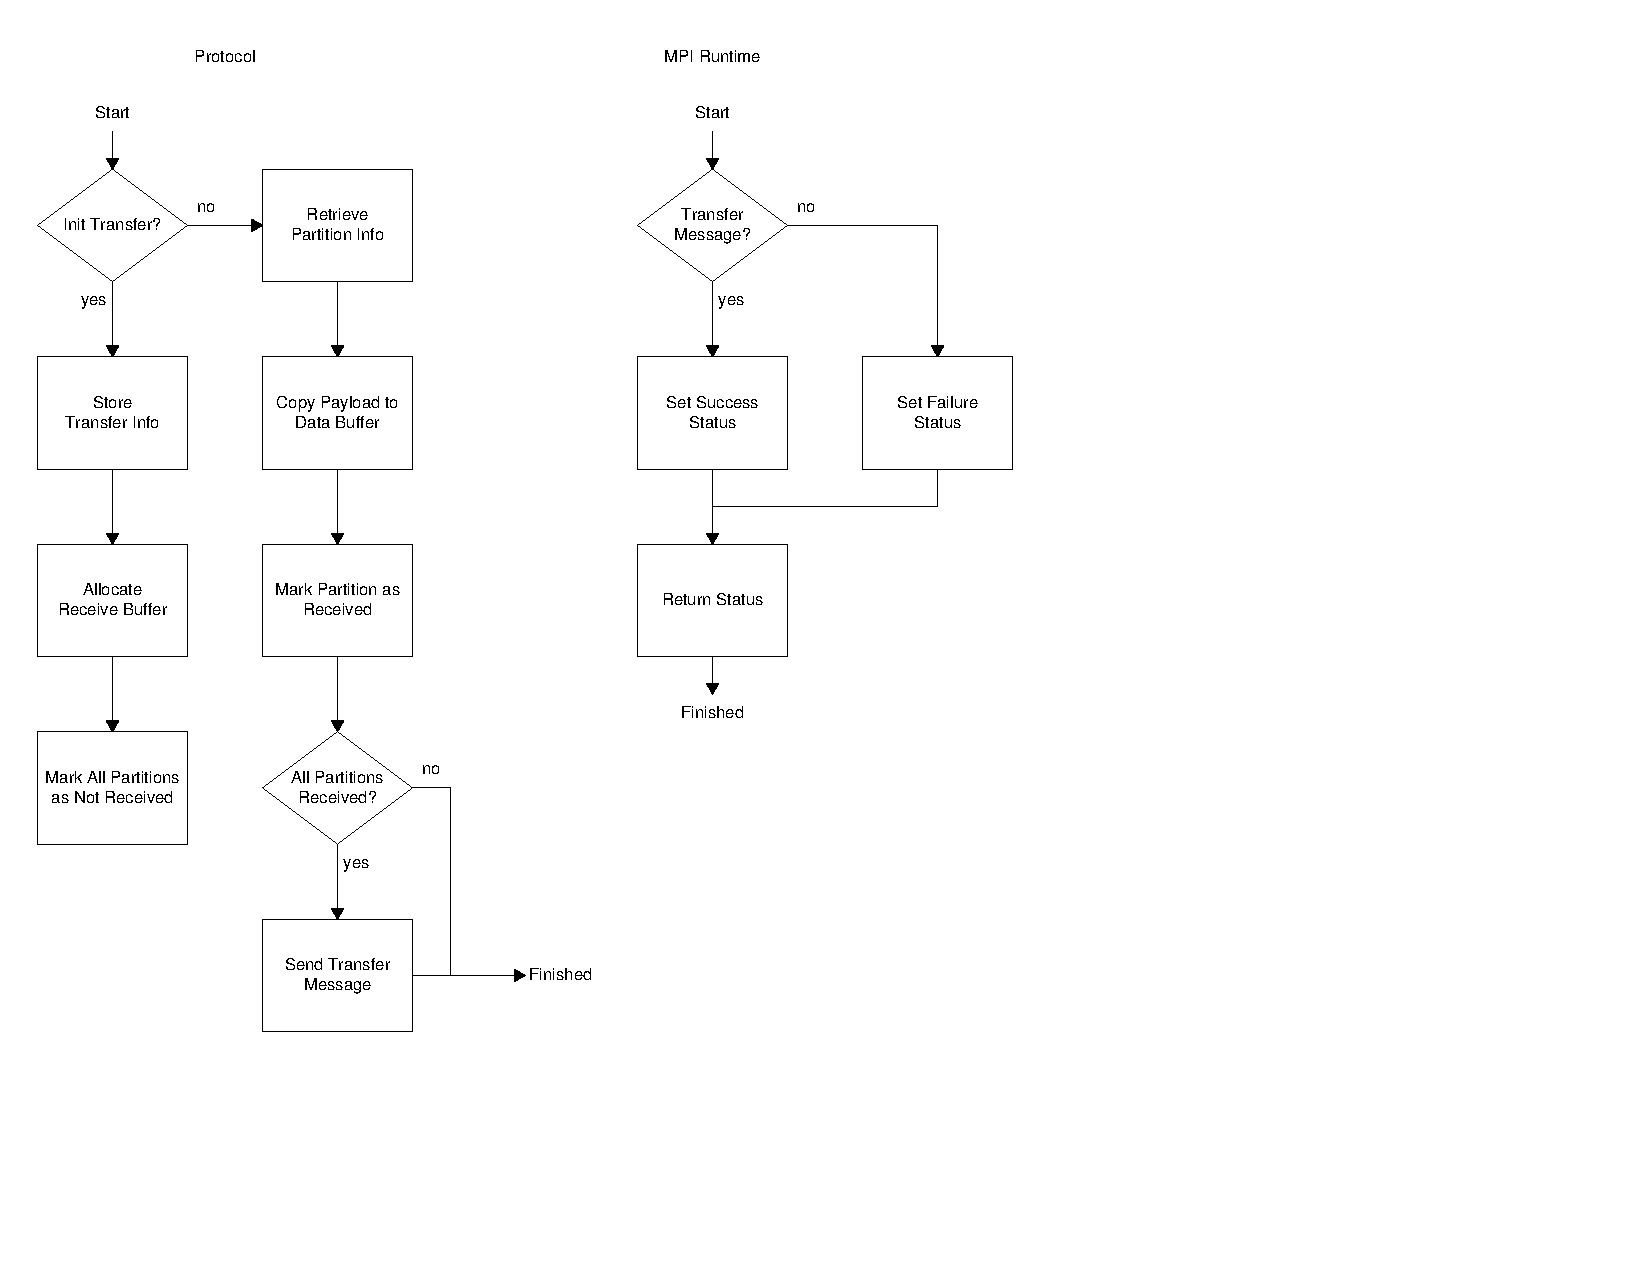
\includegraphics{API/Figures/api-irecv_process_diagram.pdf}
		\caption{Asynchronous Receive Process Diagram}
		\label{fig:api:irecv_process_diagram}
	\end{centering}
\end{figure}

The root node is used to coordinate barriers. When an application calls a barrier, it sends an application control protocol command to the root. Like all MPI calls, this one must provide guaranteed delivery. The ACK sequence step notifies the sender when the root has received the message so the sender knows to stop retrying. This is also sent in the form of a mail message. Once the sender has received a barrier reached message (via another application control protocol command), it returns control to the application. On the root side, a barrier counter is initialized when the first barrier message is received. Each additional message received increments the counter. Once the counter equals the number of other nodes in the network, the root sends an application control protocol command to the other nodes letting them know the barrier has been reached. This process is shown in Figure \ref{fig:api:barrier_process_diagram}.

\begin{figure}[ptb]
	\begin{centering}
		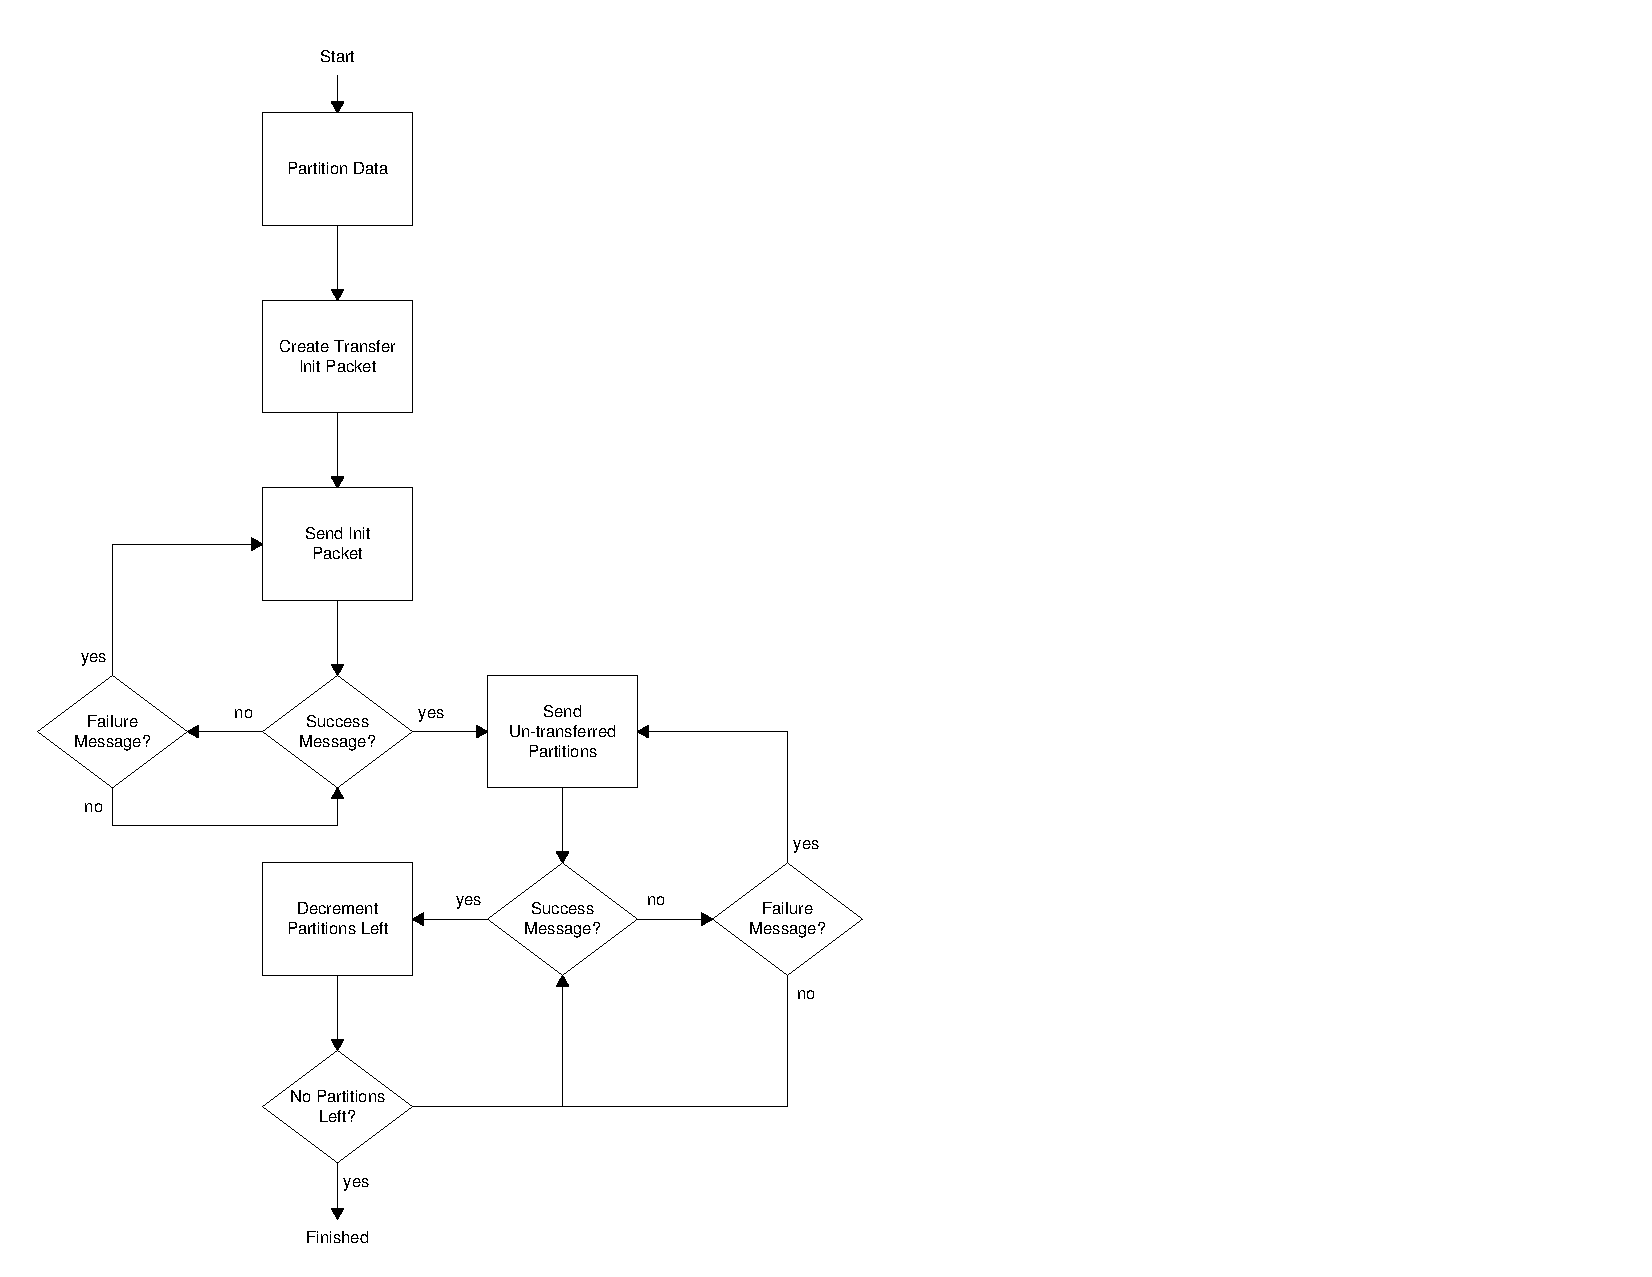
\includegraphics{API/Figures/api-send_process_diagram.pdf}
		\caption{Barrier Process Diagram}
		\label{fig:api:barrier_process_diagram}
	\end{centering}
\end{figure}

\section{Results}\label{sec:api:results}

A sample parallel algorithm was written that tests the MPI implementation. Discrete convolution was chosen as the algorithm to implement because it requires less memory than matrix multiple (a parallel computing staple) but is still embarrassingly parallel. Choosing an embarrassingly parallel algorithm is critical because performance loss due to the parallel system is much more significant than performance loss due to the algorithm itself. Given two discrete signals $f[n]$ and $g[n]$, discrete convolution is defined as:
\[
f[n]*g[n]=\sum_{m=-\infty}^\infty f[m]\cdot g[n-m]
\]
An important aspect of this algorithm is that there are no dependencies between $f[n]*g[n]$ and $f[n+1]*g[n+1]$ or $f[m]\cdot g[n-m]$ and $f[m+1]\cdot g[n-(m+1)]$. This property makes the algorithm embarrassingly parallel, as well as simple to implement. The algorithm is implemented twice: once as a sequential algorithm and once as a parallel algorithm. It is important to compare the parallel speed to the speed of a truly sequential algorithm when measuring speedup and efficiency because the baseline overhead implicit in parallel algorithms can favorably skew the results if the parallel algorithm with a single node is used for the sequential speed. The algorithms are implemented as nested \lstinline$for$ loops, with the parallel algorithm distributing the outer for loop to the participating nodes. The full code is shown in Appendix \ref{sec:appendix:mpi_test_code}. The algorithm is run with $\left| f[n]\right| =\left| g[n]\right| =\left\{ 100,200,300,400,500,600,700\right\}$ to test granularity, and with the number of nodes $n=\left\{ 1,2,3,4,5,6,7\right\}$ to test scalability. The speedup is shown in Figure \ref{fig:api:convolution_speedup} and the efficiency is shown in Figure \ref{fig:api:convolution_efficiency}. 2-D graphs showing the speedup and efficiency for each data size can be found in Appendix \ref{sec:appendix:mpi_results}.

\begin{landscape}
	\begin{figure}[p]
		\begin{centering}
			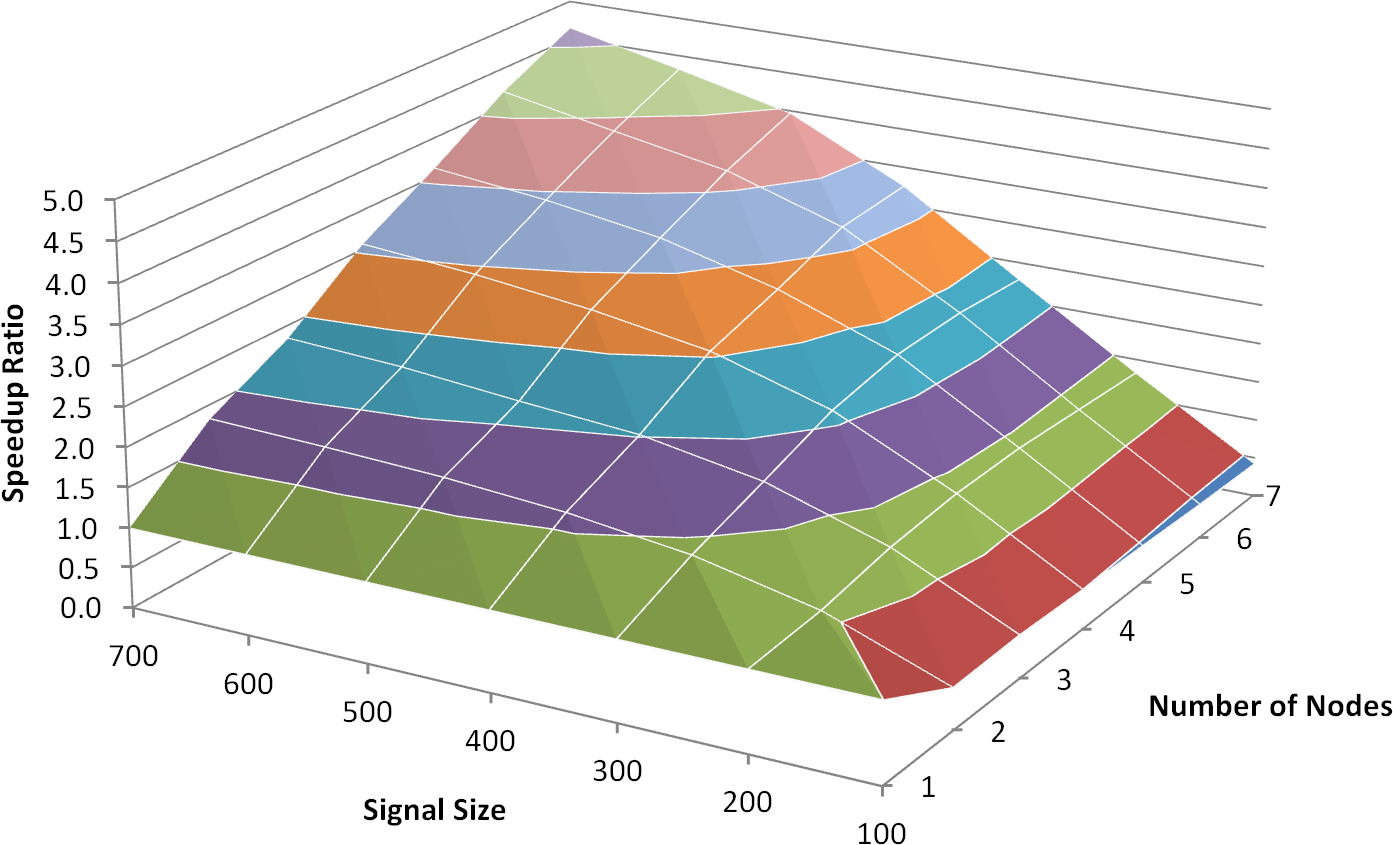
\includegraphics[width=8.5in]{API/Figures/api-convolution_speedup.png}
			\caption{Speedup Ratio for the Convolution Test}
			\label{fig:api:convolution_speedup}
		\end{centering}
	\end{figure}
\end{landscape}

\begin{landscape}
	\begin{figure}[p]
		\begin{centering}
			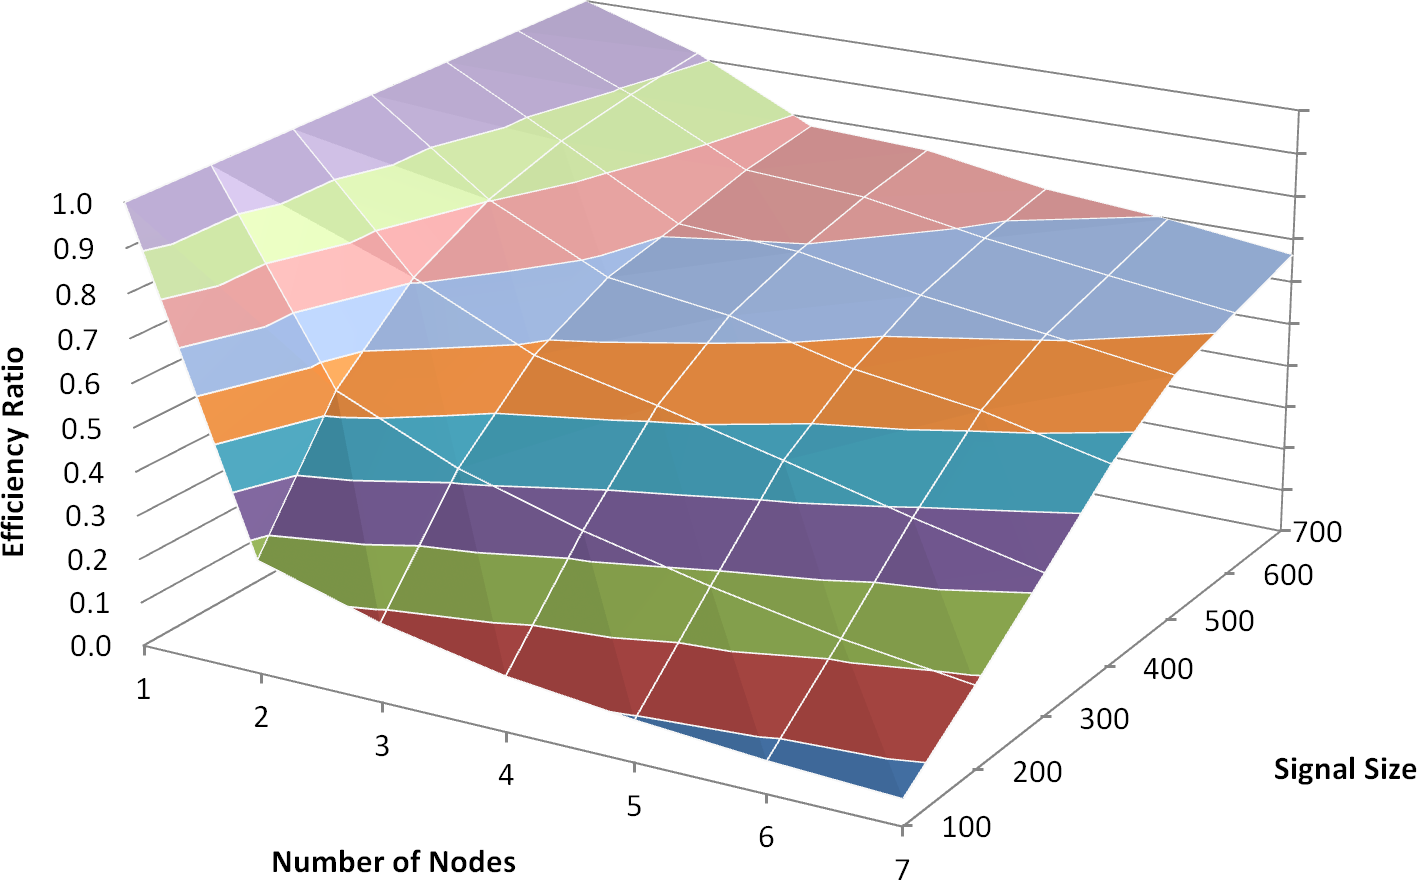
\includegraphics[width=8.5in]{API/Figures/api-convolution_efficiency.png}
			\caption{Efficiency Ratio for the Convolution Test}
			\label{fig:api:convolution_efficiency}
		\end{centering}
	\end{figure}
\end{landscape}

The results shown are pretty expected. The code is pretty slow, overall, but is consistent with the findings in the previous chapters. These results show that the prototype, as implemented on the F2808, is effective for coarse-grained parallel algorithms, but not for fine-grained parallel algorithms. Figure \ref{fig:api:convolution_speedup} shows that there is a consistent, if not quite linear, speedup as the number of nodes grow when working with large signal sizes. As the signal size decreases, the speedup and efficiency also decrease. At the other end with 100 element signals, the results are atrocious, as one would expect with a relatively fine-grained algorithm running on a system such as this. An interesting, albeit expected, a phenomenon occurs with the 100 element signal size in relation to the number of nodes: the speedup drops markedly from one node to two. This drop is due to the baseline overhead implicit in the parallel algorithm, and with this small of a signal size the overhead becomes dominant.

\section{Future Work}\label{sec:api:future_work}

There is one MPI function that is notably absent: \lstinline$MPI_Isend$. This method could not be developed easily with the given threading framework. \lstinline$MPI_Isend$ requires a thread of execution that is independent of the main application to handle the guaranteed delivery of its payload. It is not reasonable to implement these mechanisms in the \lstinline$MPI_Test$ code and the protocol stack, unlike \lstinline$MPI_Irecv$, because sending takes an active role in the transmission process, as opposed to receiving's passive role. Code was actually written to enable this behavior, but it had to be removed due to problems with DSP/BIOS. The fix is to implement a thread that time-slices with the running application, but unfortunately DSP/BIOS is atrocious at time-slicing. Once a different RTOS is utilized, it will be possible to re-introduce the \lstinline$MPI_Isend$ code. DSP/BIOS and the problems incurred are discussed further in Chapter \ref{sec:conclusions:future_work}.

There are a few other functions that would be useful if implemented. \lstinline$MPI_Bcast$ would be useful, but needs broadcast support from the network layer before this is possible. Full support for communicators could also be beneficial.

\section{Conclusions}\label{sec:api:conclusions}

In this chapter, a background to parallel was given. A subset of MPI was presented that runs on the prototype toolkit. It offers basic support for sending and receiving, synchronization, and other system and support related activities. The code has been tested using a parallel implementation of discrete convolution. The speedup and efficiency results show that the prototype is effective when used for coarse-grained parallel algorithms, but expectedly is poor at handling finer grained parallel algorithms.



